% Options for packages loaded elsewhere
\PassOptionsToPackage{unicode}{hyperref}
\PassOptionsToPackage{hyphens}{url}
%
\documentclass[
]{book}
\usepackage{lmodern}
\usepackage{amssymb,amsmath}
\usepackage{ifxetex,ifluatex}
\ifnum 0\ifxetex 1\fi\ifluatex 1\fi=0 % if pdftex
  \usepackage[T1]{fontenc}
  \usepackage[utf8]{inputenc}
  \usepackage{textcomp} % provide euro and other symbols
\else % if luatex or xetex
  \usepackage{unicode-math}
  \defaultfontfeatures{Scale=MatchLowercase}
  \defaultfontfeatures[\rmfamily]{Ligatures=TeX,Scale=1}
\fi
% Use upquote if available, for straight quotes in verbatim environments
\IfFileExists{upquote.sty}{\usepackage{upquote}}{}
\IfFileExists{microtype.sty}{% use microtype if available
  \usepackage[]{microtype}
  \UseMicrotypeSet[protrusion]{basicmath} % disable protrusion for tt fonts
}{}
\makeatletter
\@ifundefined{KOMAClassName}{% if non-KOMA class
  \IfFileExists{parskip.sty}{%
    \usepackage{parskip}
  }{% else
    \setlength{\parindent}{0pt}
    \setlength{\parskip}{6pt plus 2pt minus 1pt}}
}{% if KOMA class
  \KOMAoptions{parskip=half}}
\makeatother
\usepackage{xcolor}
\IfFileExists{xurl.sty}{\usepackage{xurl}}{} % add URL line breaks if available
\IfFileExists{bookmark.sty}{\usepackage{bookmark}}{\usepackage{hyperref}}
\hypersetup{
  pdftitle={Introdução ao R},
  pdfauthor={Raimundo Marciano de Freitas Neto},
  hidelinks,
  pdfcreator={LaTeX via pandoc}}
\urlstyle{same} % disable monospaced font for URLs
\usepackage{color}
\usepackage{fancyvrb}
\newcommand{\VerbBar}{|}
\newcommand{\VERB}{\Verb[commandchars=\\\{\}]}
\DefineVerbatimEnvironment{Highlighting}{Verbatim}{commandchars=\\\{\}}
% Add ',fontsize=\small' for more characters per line
\usepackage{framed}
\definecolor{shadecolor}{RGB}{248,248,248}
\newenvironment{Shaded}{\begin{snugshade}}{\end{snugshade}}
\newcommand{\AlertTok}[1]{\textcolor[rgb]{0.94,0.16,0.16}{#1}}
\newcommand{\AnnotationTok}[1]{\textcolor[rgb]{0.56,0.35,0.01}{\textbf{\textit{#1}}}}
\newcommand{\AttributeTok}[1]{\textcolor[rgb]{0.77,0.63,0.00}{#1}}
\newcommand{\BaseNTok}[1]{\textcolor[rgb]{0.00,0.00,0.81}{#1}}
\newcommand{\BuiltInTok}[1]{#1}
\newcommand{\CharTok}[1]{\textcolor[rgb]{0.31,0.60,0.02}{#1}}
\newcommand{\CommentTok}[1]{\textcolor[rgb]{0.56,0.35,0.01}{\textit{#1}}}
\newcommand{\CommentVarTok}[1]{\textcolor[rgb]{0.56,0.35,0.01}{\textbf{\textit{#1}}}}
\newcommand{\ConstantTok}[1]{\textcolor[rgb]{0.00,0.00,0.00}{#1}}
\newcommand{\ControlFlowTok}[1]{\textcolor[rgb]{0.13,0.29,0.53}{\textbf{#1}}}
\newcommand{\DataTypeTok}[1]{\textcolor[rgb]{0.13,0.29,0.53}{#1}}
\newcommand{\DecValTok}[1]{\textcolor[rgb]{0.00,0.00,0.81}{#1}}
\newcommand{\DocumentationTok}[1]{\textcolor[rgb]{0.56,0.35,0.01}{\textbf{\textit{#1}}}}
\newcommand{\ErrorTok}[1]{\textcolor[rgb]{0.64,0.00,0.00}{\textbf{#1}}}
\newcommand{\ExtensionTok}[1]{#1}
\newcommand{\FloatTok}[1]{\textcolor[rgb]{0.00,0.00,0.81}{#1}}
\newcommand{\FunctionTok}[1]{\textcolor[rgb]{0.00,0.00,0.00}{#1}}
\newcommand{\ImportTok}[1]{#1}
\newcommand{\InformationTok}[1]{\textcolor[rgb]{0.56,0.35,0.01}{\textbf{\textit{#1}}}}
\newcommand{\KeywordTok}[1]{\textcolor[rgb]{0.13,0.29,0.53}{\textbf{#1}}}
\newcommand{\NormalTok}[1]{#1}
\newcommand{\OperatorTok}[1]{\textcolor[rgb]{0.81,0.36,0.00}{\textbf{#1}}}
\newcommand{\OtherTok}[1]{\textcolor[rgb]{0.56,0.35,0.01}{#1}}
\newcommand{\PreprocessorTok}[1]{\textcolor[rgb]{0.56,0.35,0.01}{\textit{#1}}}
\newcommand{\RegionMarkerTok}[1]{#1}
\newcommand{\SpecialCharTok}[1]{\textcolor[rgb]{0.00,0.00,0.00}{#1}}
\newcommand{\SpecialStringTok}[1]{\textcolor[rgb]{0.31,0.60,0.02}{#1}}
\newcommand{\StringTok}[1]{\textcolor[rgb]{0.31,0.60,0.02}{#1}}
\newcommand{\VariableTok}[1]{\textcolor[rgb]{0.00,0.00,0.00}{#1}}
\newcommand{\VerbatimStringTok}[1]{\textcolor[rgb]{0.31,0.60,0.02}{#1}}
\newcommand{\WarningTok}[1]{\textcolor[rgb]{0.56,0.35,0.01}{\textbf{\textit{#1}}}}
\usepackage{longtable,booktabs}
% Correct order of tables after \paragraph or \subparagraph
\usepackage{etoolbox}
\makeatletter
\patchcmd\longtable{\par}{\if@noskipsec\mbox{}\fi\par}{}{}
\makeatother
% Allow footnotes in longtable head/foot
\IfFileExists{footnotehyper.sty}{\usepackage{footnotehyper}}{\usepackage{footnote}}
\makesavenoteenv{longtable}
\usepackage{graphicx,grffile}
\makeatletter
\def\maxwidth{\ifdim\Gin@nat@width>\linewidth\linewidth\else\Gin@nat@width\fi}
\def\maxheight{\ifdim\Gin@nat@height>\textheight\textheight\else\Gin@nat@height\fi}
\makeatother
% Scale images if necessary, so that they will not overflow the page
% margins by default, and it is still possible to overwrite the defaults
% using explicit options in \includegraphics[width, height, ...]{}
\setkeys{Gin}{width=\maxwidth,height=\maxheight,keepaspectratio}
% Set default figure placement to htbp
\makeatletter
\def\fps@figure{htbp}
\makeatother
\setlength{\emergencystretch}{3em} % prevent overfull lines
\providecommand{\tightlist}{%
  \setlength{\itemsep}{0pt}\setlength{\parskip}{0pt}}
\setcounter{secnumdepth}{5}
\usepackage{booktabs}
\usepackage[]{natbib}
\bibliographystyle{apalike}

\title{Introdução ao R}
\author{Raimundo Marciano de Freitas Neto}
\date{2021-04-01}

\begin{document}
\maketitle

{
\setcounter{tocdepth}{1}
\tableofcontents
}
\hypertarget{boas-vindas}{%
\chapter{Boas vindas}\label{boas-vindas}}

O curso será composto por módulos teóricos e práticos e terá duração de XX horas, distribuídas em XX semanas, conforme o seguinte cronograma:

\begin{itemize}
\tightlist
\item
  S01 00-00 a 00-00 Introdução
\item
  S02 00-00 a 00-00 Introdução
\item
  S03 00-00 a 00-00 Introdução
\item
  S04 00-00 a 00-00 Introdução
\item
  S05 00-00 a 00-00 Introdução
\item
  S06 00-00 a 00-00 Introdução
\end{itemize}

O curso é essencialmente assíncrono e a frequência será registrada de acordo com a entrega das atividades nos prazos assinalados.

Nas XX-feiras, das XXh às XXhXX, teremos um encontro síncrono para dúvidas via Google Meet.

\hypertarget{intro}{%
\chapter{O que é o R?}\label{intro}}

R é uma linguagem de programação muito utilizada para o desenvolvimento de estatísticas e cálculos matemáticos. Entretanto, enquanto linguagem de programação, ela possui muitos usos, como a raspagem de sites, a automatização de download de arquivos, e a produção de dashboards e relatórios, sendo útil para a coleta de dados e para o reporte das análises, além de ser gratuita.

Mas o que significa ser uma linguagem de programação? Basicamente, você irá dar ordens ao computador por meio de comandos. A vantagem de aprender a estruturar os comandos (ao invés de usar um programa estatístico já consolidado, como o Stata) é que você pode customizar a vontade suas análises. Os programas estatísticos trazem muitas opções pré-prontas. Por exemplo, no Stata é comum que você possa clicar em uma janela e solicitar um quadro com as estatísticas descritivas (média, moda, mediana) de um banco de dados. Entretanto, qualquer funcionalidade fora do padrão oferecido por aqueles pacotes precisará ser gerada pelo próprio usuário (e quando você usa algum recurso como o ssc install é porque alguém gastou um tempinho fazendo isso).

Aliás, o Python (outra linguagem de programação) possui funcionalidades bem similares ao R, embora o modo de escrever os programas seja bem diferente. Imagine que o Português e o Espanhol têm o mesmo propósito - a comunicação - e que mesmo tendo uma mesma raiz (e inclusive diversos vocábulos bem parecidos), possuem algumas regras estruturais bem diferentes, o que inclui, por exemplo, as regras de acentuação e o som produzidos pelas letras: qual a diferença de cajá (PT-BR) para caja (ES); qual a diferença de pastel (PT-BR) para pastel (ES)?

É preferível que o analista iniciante dedique-se a uma das duas (R ou Python). Posteriormente, aprender a outra (ou mais alguma que esteja despontando no mercado, como a Julia) será uma tarefa bem mais simples. Isso se deve ao fato de que diversos elementos da programação se repetem entre as diferentes linguagens, especialmente os conceitos. Um IF tem o mesmo propósito em R ou em Python ou em Java ou em C++, embora a forma como você deve explicar ao computador o que fazer com esse IF será bem diferente em cada linguagem.

\hypertarget{scripts}{%
\section{Scripts}\label{scripts}}

\hypertarget{instalando-o-r}{%
\section{Instalando o R}\label{instalando-o-r}}

O R é instalado como um programa normal. Primeiro, você deve acessar a página do \href{https://cran.r-project.org/mirrors.html}{R Project}. Há vários links para baixar. Todos funcionam e disponibilizam os mesmos arquivos, mas sugere-se clicar no local mais próximo ao que você se encontra.

Na nova página, clique em Download R for Windows. Depois, clique em base. Caso você queira baixar a versão mais recente, clique em Download R xxx for Windows. Caso você prefira uma versão mais antiga, clique em Previous releases (fica um pouco abaixo, na seção Other Builds).

Alternativamente, \href{https://vps.fmvz.usp.br/CRAN/bin/windows/base/release.html}{clique aqui}.

\begin{figure}
\centering
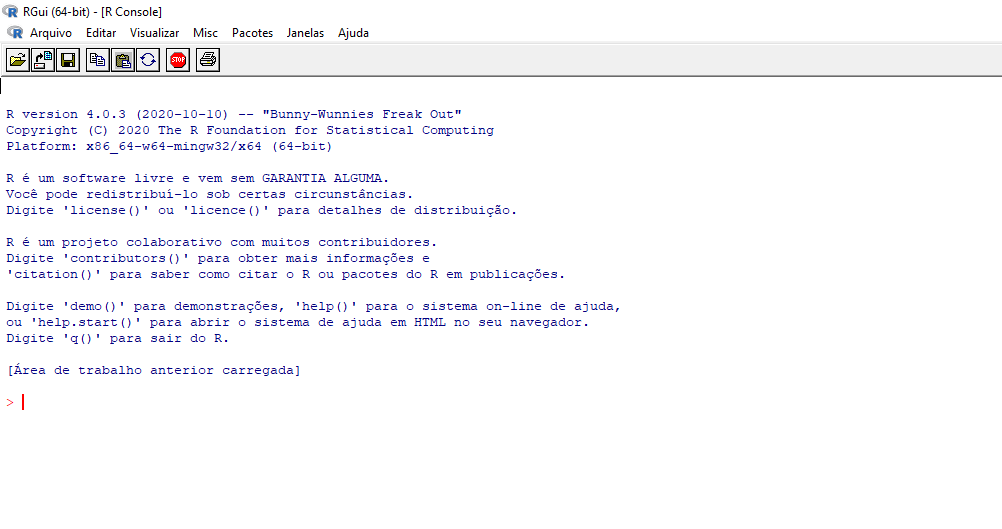
\includegraphics{r-gui.PNG}
\caption{Aparência do R-GUI}
\end{figure}

Na parte superior, é possível visualizar a versão do R que está sendo executada. Nem sempre é interessante, para o programador novato, usar a última versão disponível, porque ela ainda pode conter alguns bugs. Por isso, mesmo que a versão mais atual seja a 4.0.4, pode ser interessante nos mantermos na 4.0.3 ou até mesmo na 3.6.3.

Na linha iniciada por \(>\) podemos dar instruções ao R. Por exemplo, digite 1+1 e depois aperte ENTER.

\begin{Shaded}
\begin{Highlighting}[]
\DecValTok{1}\OperatorTok{+}\DecValTok{1}
\end{Highlighting}
\end{Shaded}

\begin{verbatim}
## [1] 2
\end{verbatim}

O R executou a soma solicitada e retornou o resultado.

\hypertarget{r-studio}{%
\section{R Studio}\label{r-studio}}

O R Studio é um programa que permite trabalhar o R de forma aprimorada. Ele é o que os desenvolvedores chamada de Ambiente Integrado de Desenvolvimento (ou Integrated Development Environment (IDE), no original). Já tendo instalado o R, que fornece a base da linguagem de programação e a interface básica com o computador, podemos agora instalar o R Studio.

Primeiramente acesse o site do \href{https://www.rstudio.com/products/rstudio/download/\#download}{R Studio}. Embora existam versões pagas com recursos interessantes, todos os recursos necessários ao programador iniciante estão incluídos na versão gratuita. Clique no botão DOWNLOAD R STUDIO FOR WINDOWS. Depois do download concluído, instale o programa na sua máquina normalmente. O R Studio automaticamente identifica o R-base instalado na sua máquina (é realmente necessário já ter instalado o R antes!).

\hypertarget{r-nas-nuvens}{%
\section{R nas Nuvens}\label{r-nas-nuvens}}

\hypertarget{variuxe1veis}{%
\chapter{Variáveis}\label{variuxe1veis}}

Os dados são inseridos no R como variáveis. Eles podem ser importados (trazidos de um arquivo para o R) ou digitados no próprio console. Quando você deseja armazenar um valor na memória, você deve atribuí-lo, usando o sinal = ou \textless-.

\begin{Shaded}
\begin{Highlighting}[]
\NormalTok{x =}\StringTok{ }\DecValTok{1}
\KeywordTok{print}\NormalTok{(x)}
\end{Highlighting}
\end{Shaded}

\begin{verbatim}
## [1] 1
\end{verbatim}

\begin{Shaded}
\begin{Highlighting}[]
\NormalTok{y <-}\StringTok{ }\DecValTok{1}\OperatorTok{+}\DecValTok{1}
\NormalTok{y}
\end{Highlighting}
\end{Shaded}

\begin{verbatim}
## [1] 2
\end{verbatim}

\begin{Shaded}
\begin{Highlighting}[]
\NormalTok{texto =}\StringTok{ "Esse é um texto. Observe as aspas duplas"}
\NormalTok{assim =}\StringTok{ 'Também podem ser usadas aspas simples'}
\NormalTok{sugestao =}\StringTok{ 'Use aspas simples sempre que "possível" para delimitar a variável. Os }
\StringTok{textos em português costumam usadas aspas duplas.'}
\KeywordTok{print}\NormalTok{(sugestao)}
\end{Highlighting}
\end{Shaded}

\begin{verbatim}
## [1] "Use aspas simples sempre que \"possível\" para delimitar a variável. Os \ntextos em português costumam usadas aspas duplas."
\end{verbatim}

\begin{Shaded}
\begin{Highlighting}[]
\KeywordTok{writeLines}\NormalTok{(sugestao)}
\end{Highlighting}
\end{Shaded}

\begin{verbatim}
## Use aspas simples sempre que "possível" para delimitar a variável. Os 
## textos em português costumam usadas aspas duplas.
\end{verbatim}

O R é uma linguagem que automaticamente reconhece o tipo do dado que foi inserido. Por uma questão de comparação, se você estivesse usando uma linguagem \emph{tipada}, como o C++, você precisaria declarar explicitamente o tipo da variável que está sendo criada. Assim, seria um erro você criar uma variável usando

\begin{Shaded}
\begin{Highlighting}[]
\NormalTok{dois =}\StringTok{ }\DecValTok{2}
\end{Highlighting}
\end{Shaded}

O C++ não entende o que você está querendo dizer com isso. Você precisaria informar que existe uma variável do tipo \emph{integer} (simplesmente \emph{int}) chamada \emph{dois} e cujo valor é o número inteiro 2. Outra particularidade do R é que as linhas de código não precisam ser finalizadas com um ponto-e-vírgula (;), como acontece no C++.

\begin{Shaded}
\begin{Highlighting}[]
\NormalTok{int dois =}\StringTok{ }\DecValTok{2}\NormalTok{;}
\end{Highlighting}
\end{Shaded}

Além disso, as variáveis em R são mutáveis, inclusive quanto ao tipo. Isso quer dizer que uma vez definidas (ou atribuídas), podem ter seus valores e tipo modificados. Assim, uma variável que antes tinha um número, pode passar a ter um texto ou um booleano.

\begin{Shaded}
\begin{Highlighting}[]
\CommentTok{# se a variavel receber um número (integer)}
\NormalTok{dois <-}\StringTok{ }\DecValTok{2}
\CommentTok{# e depois receber um texto}
\NormalTok{dois <-}\StringTok{ "dois"}
\CommentTok{# seu conteúdo e seu tipo estarão de acordo com a última atribuição}
\KeywordTok{print}\NormalTok{(dois)}
\end{Highlighting}
\end{Shaded}

\begin{verbatim}
## [1] "dois"
\end{verbatim}

Por fim, para o R a indentação não é relevante. Há linguagens de programação em que a posição relativa das linhas de código é essencial para determinar se elas fazem parte de um bloco ou não. No R, os blocos são definidos com o uso de chaves (\{ \}). Ainda iremos explorar com detalhes o uso das condicionais, mas podemos ilustrar o seguinte caso: se o resultado for maior que zero, então, sim, tivemos lucro; caso contrário, não tivemos.

\begin{Shaded}
\begin{Highlighting}[]
\NormalTok{resultado <-}\StringTok{ }\DecValTok{3000}

\CommentTok{#se o resultado for maior que zero}
\ControlFlowTok{if}\NormalTok{ (resultado }\OperatorTok{>}\StringTok{ }\DecValTok{0}\NormalTok{) \{ }
  \CommentTok{# informe: "Tivemos Lucro!"}
  \KeywordTok{print}\NormalTok{(}\StringTok{"Tivemos Lucro!"}\NormalTok{) }
  \CommentTok{# caso contrário}
\NormalTok{\} }\ControlFlowTok{else}\NormalTok{ \{  }
  \CommentTok{# informe: "Deu ruim :( "}
  \KeywordTok{print}\NormalTok{(}\StringTok{"Deu ruim :("}\NormalTok{) }
\NormalTok{\}}
\end{Highlighting}
\end{Shaded}

\begin{verbatim}
## [1] "Tivemos Lucro!"
\end{verbatim}

No R, esse alinhamento é apenas um facilitador de leitura do código. Se o código estiver organizado, as pessoas terão mais facilidade em entendê-lo. O código a seguir tem exatamente a mesma funcionalidade.

\begin{Shaded}
\begin{Highlighting}[]
\NormalTok{resultado <-}\StringTok{ }\DecValTok{3000}
\ControlFlowTok{if}\NormalTok{ (resultado }\OperatorTok{>}\StringTok{ }\DecValTok{0}\NormalTok{) \{ }\KeywordTok{print}\NormalTok{(}\StringTok{"Tivemos Lucro!"}\NormalTok{) \} }\ControlFlowTok{else}\NormalTok{ \{}\KeywordTok{print}\NormalTok{(}\StringTok{"Deu ruim :("}\NormalTok{)\}}
\end{Highlighting}
\end{Shaded}

\begin{verbatim}
## [1] "Tivemos Lucro!"
\end{verbatim}

Embora seja verdade que o espaço ocupado está menor, quando o código começa a adquirir um alto grau de complexidade, torna-se muito desejável que ele esteja melhor organizado e, preferencialmente, comentado.

No Python, onde a identação faz diferença, o código precisaria seguir uma estrutura baseada em espaços, sendo desnecessário o uso das chaves.

\begin{Shaded}
\begin{Highlighting}[]
\CommentTok{#se o resultado for maior que zero}
\ControlFlowTok{if}\NormalTok{ (resultado }\OperatorTok{>} \DecValTok{0}\NormalTok{):  }
  \CommentTok{# informe: "Tivemos Lucro!"}
  \BuiltInTok{print}\NormalTok{(}\StringTok{"Tivemos Lucro!"}\NormalTok{) }
\ControlFlowTok{else}\NormalTok{:  }
  \CommentTok{# informe: "Deu ruim :( "}
  \BuiltInTok{print}\NormalTok{(}\StringTok{"Deu ruim :("}\NormalTok{) }
\end{Highlighting}
\end{Shaded}

No Python, portanto, o que importa para definir que o print(``Tivemos Lucro!'') está associado ao if(resultado \textgreater{} 0) é o fato de não haver nenhum espaço entre a margem da página e o if; e o fato de haver quatro espaços entre a margem da página e o print. Isso faz com que esse print esteja subordinado ao if; assim como, o segundo print (que também está mais recuado) é subordinado ao else (que não tem recuo).

\hypertarget{numuxe9ricas}{%
\section{Numéricas}\label{numuxe9ricas}}

O R possui uma abordagem simplificada para o tratamento de números. Em tese, na computação os números possuem várias classificações, como: inteiro (integer), que não admitem casas decimais, e ponto-flutuantes (float), que possuem casas decimais. Portanto, 3 pode ser um integer, enquanto 3,5 não pode (tem um dígito após a vírgula). Ainda há mais algumas classificações, como o double e o long, mas o integer e o float são suficientes para o que precisamos discutir.

Basicamente existem os inteiros (integers) e os ponto-flutuantes (float). O integer não admite casas decimais, sendo usado para eventos contáveis, como a quantidade de vezes que algo ocorreu. O float admite casas decimais, sendo indicado para representar valores monetários.

Veja, por exemplo, o caso da idade. Se a idade for calculada como a diferença entre anos (2021 - 1988 = 33), o resultado será um número inteiro, que pode ser representado por um integer. Contudo, se uma idade como 12,5 anos for admitida, então será necessário trabalhar com float. Se você está lendo isso em fevereiro, pense na representação correta da idade de alguém que nasceu em dezembro.

Raramente, isso será uma preocupação. Como dito, o R faz a análise automática e, por padrão, categoriza os números dentro do tipo numeric, que aceita tanto integers como floats. Eventualmente, algum erro pode acontecer, como haver algum canto na planilha que está sendo importada em que foi digitado 2x20 ao invés de 2020. Quando o R tentasse ler esse valor (2x20), ele reconheceria um caractere que não é um número e automaticamente tentaria entender isso como sendo um texto.

\hypertarget{textuais}{%
\section{Textuais}\label{textuais}}

Para inserir um caractere, uma palavra ou uma frase, é necessário o uso de aspas simples ou duplas. Como no português é comum o uso de aspas duplas, é interessante o uso de aspas simples no R. Isso se deve ao fato de que se você precisar eventualmente incluir as aspas duplas, elas podem ficar dentro das aspas simples.

Por exemplo, é aceitável:

\begin{Shaded}
\begin{Highlighting}[]
\NormalTok{texto1 =}\StringTok{ 'Ela disse: "Ok".'}
\NormalTok{texto2 =}\StringTok{ 'E eu respondi "Certo".'}
\KeywordTok{writeLines}\NormalTok{(}\KeywordTok{c}\NormalTok{(texto1, texto2))}
\end{Highlighting}
\end{Shaded}

\begin{verbatim}
## Ela disse: "Ok".
## E eu respondi "Certo".
\end{verbatim}

Perceba que as aspas simples estão funcionando apenas como delimitadores. Estão dizendo que tudo que está dentro delas faz parte de um mesmo texto, inclusive as aspas duplas.

\begin{Shaded}
\begin{Highlighting}[]
\NormalTok{texto3 <-}\StringTok{ "Ela disse: "}\NormalTok{Ok}\StringTok{"."}
\end{Highlighting}
\end{Shaded}

O texto3 seria problemático para o R. Assim que ele identifica as primeiras aspas, ele passa a esperar um texto. Quando aparecem mais aspas, ele entende que o texto foi encerrado e não pretende continuar lendo o que vem depois. Com isso, ele estranha que tenha mais texto logo após (Ok``.'')

\hypertarget{numuxe9rica-ou-textual}{%
\subsection{Numérica ou textual?}\label{numuxe9rica-ou-textual}}

O CNPJ de uma empresa é composto por 14 dígitos numéricos (0 a 9), separados por alguns marcadores (pontos, barras e traços). Por exemplo, pode ser 12.345.678/0001-19. Para guardar essa informação como uma variável numérica, você precisaria omitir as marcações, digitando 12345678000119. Entretanto, existe aqui um problema: o caso dos CNPJs iniciados por 0. Se há um 0 no início do número, ele é sempre ignorado. Por exemplo, 02 sempre será salvo na memória como 2, porque o zero à esquerda, na Matemática, não tem função.

Pensando nisso, pode ser mais interessante salvar o CNPJ como uma variável textual.

\begin{Shaded}
\begin{Highlighting}[]
\NormalTok{cnpj <-}\StringTok{ "12.345.678/0001-19"}
\end{Highlighting}
\end{Shaded}

Com isso não são perdidos os marcadores. Perceba, por fim, que o tratamento desse ``número'' como texto não tem implicações sobre a análise estatística dos dados. O CNPJ não é um número sobre o qual você realiza operações matemáticas. Você não calcula a média,a moda ou a mediana dos CNPJs e nem cria um gráfico de CNPJs. Ele é um identificador da empresa, tal qual o nome dela.

No caso de pessoas físicas, o mesmo raciocínio vale para o CPF.

\begin{quote}
Exceção: os dois últimos dígitos do CNPJ (e do CPF) são um código verificador. Alguns formulários cadastrais usam esses dois últimos dígitos para conferir se o campo foi preenchido corretamente. Essa conferência é feita a partir de um cálculo matemático; logo, há casos específicos em que mesmo o CNPJ pode ser usado para algum cálculo.
\end{quote}

\hypertarget{luxf3gicas}{%
\section{Lógicas}\label{luxf3gicas}}

Em muitos casos, é importante ter variáveis que indiquem VERDADEIRO (TRUE) ou FALSO (FALSE).O tipo de variável que admite apenas esses dois valores lógicos é chamado de Booleana (boolean ou bool). Essas variáveis seguem a lógica de primeira ordem. Por exemplo, TRUE AND FALSE resulta em FALSE, enquanto TRUE OR FALSE resulta em TRUE.

\begin{Shaded}
\begin{Highlighting}[]
\CommentTok{# AND ou E é representado por &}
\KeywordTok{print}\NormalTok{(}\OtherTok{TRUE} \OperatorTok{&}\StringTok{ }\OtherTok{FALSE}\NormalTok{)}
\end{Highlighting}
\end{Shaded}

\begin{verbatim}
## [1] FALSE
\end{verbatim}

\begin{Shaded}
\begin{Highlighting}[]
\CommentTok{# OR ou OU é representado por |}
\KeywordTok{print}\NormalTok{(}\OtherTok{TRUE} \OperatorTok{|}\StringTok{ }\OtherTok{FALSE}\NormalTok{) }
\end{Highlighting}
\end{Shaded}

\begin{verbatim}
## [1] TRUE
\end{verbatim}

Variáveis lógicas podem ter muitos usos, como parâmetros em funções ou filtros para listas de dados. Por exemplo, você pode querer que o usuário informe se ele quer imprimir o relatório dos valores ao final. Nesse caso, ele deveria informar que o valor do parâmetro imprimir\_relatorio deveria ser TRUE. Caso ele não queira imprimir o relatório, deveria informar imprimir\_relatorio como FALSE.

Também podem ser usados para comparações de igualdade (==) ou desigualdade (!=).

\begin{Shaded}
\begin{Highlighting}[]
\NormalTok{dois_numero <-}\StringTok{ }\DecValTok{2}
\NormalTok{dois_texto <-}\StringTok{ "dois"}
\CommentTok{# Vamos testar de o numero dois é o mesmo que o dois "por extenso"}
\NormalTok{dois_numero }\OperatorTok{==}\StringTok{ }\NormalTok{dois_texto}
\end{Highlighting}
\end{Shaded}

\begin{verbatim}
## [1] FALSE
\end{verbatim}

\begin{Shaded}
\begin{Highlighting}[]
\CommentTok{# Vamos testar de o numero dois é diferente do dois "por extenso"}
\NormalTok{dois_numero }\OperatorTok{!=}\StringTok{ }\NormalTok{dois_texto}
\end{Highlighting}
\end{Shaded}

\begin{verbatim}
## [1] TRUE
\end{verbatim}

O R não entende que ``dois'' é a forma ``por extenso'' do número 2. Para o R, há um número 2 e há uma palavra, cujo significado o R desconhece. Então, na comparação entre esse inteiro e essa string, o R entende que há uma diferença (de tipos). Por isso, ele afirma que são diferentes (ou não iguais).

\begin{Shaded}
\begin{Highlighting}[]
\NormalTok{dois_numero <-}\StringTok{ }\DecValTok{2}
\NormalTok{dois_texto <-}\StringTok{ "2"}
\CommentTok{# Vamos testar de o numero dois é o mesmo que o dois "caractere"}
\CommentTok{# O resultado é verdadeiro porque apesar dos tipos serem diferentes, o conteúdo é o mesmo.}
\NormalTok{dois_numero }\OperatorTok{==}\StringTok{ }\NormalTok{dois_texto}
\end{Highlighting}
\end{Shaded}

\begin{verbatim}
## [1] TRUE
\end{verbatim}

Existe outro operador de igualdade (===), mas que não será tratado agora.

\hypertarget{datas}{%
\section{Datas}\label{datas}}

\begin{Shaded}
\begin{Highlighting}[]
\NormalTok{today <-}\StringTok{ }\KeywordTok{Sys.Date}\NormalTok{()}
\KeywordTok{print}\NormalTok{(today)}
\end{Highlighting}
\end{Shaded}

\begin{verbatim}
## [1] "2021-04-01"
\end{verbatim}

\begin{Shaded}
\begin{Highlighting}[]
\NormalTok{today <-}\StringTok{ }\KeywordTok{format}\NormalTok{(today, }\StringTok{"%d/%m/%Y"}\NormalTok{)}
\KeywordTok{print}\NormalTok{(today)}
\end{Highlighting}
\end{Shaded}

\begin{verbatim}
## [1] "01/04/2021"
\end{verbatim}

\begin{Shaded}
\begin{Highlighting}[]
\NormalTok{today2 <-}\StringTok{ }\KeywordTok{format}\NormalTok{(}\KeywordTok{Sys.Date}\NormalTok{(), }\StringTok{"%d/%m/%Y"}\NormalTok{)}
\KeywordTok{print}\NormalTok{(today2)}
\end{Highlighting}
\end{Shaded}

\begin{verbatim}
## [1] "01/04/2021"
\end{verbatim}

\hypertarget{estruturas-de-dados}{%
\chapter{Estruturas de Dados}\label{estruturas-de-dados}}

Pode ser desejável juntar vários valores em um único objeto gravado na memória usada pelo R. Por exemplo, você pode querer criar um objeto que contenha o nome das empresas que tiveram as maiores ofertas públicas iniciais na bolsa de valores brasileira em 2020; ou você pode querer a relação dos nomes e dos valores. Dependendo dos tipos de dados envolvidos, a forma de fazer isso pode mudar.

\begin{quote}
O R possui o conceito de objetos, que são estruturas especializadas e que podem conter tanto os valores dos dados quanto atributos. Quando você declara uma variável simples (a = 5) ou (b = ``eu''), os atributos não são importantes - é fácil ter certeza que dentro da variável haverá um valor que a representa. Contudo, em estruturas mais complexas, com muitas linhas e colunas, é importante, por exemplo, que as colunas tenham nomes (atributos), a fim de facilitar a identificação.
\end{quote}

\hypertarget{vetores}{%
\section{Vetores}\label{vetores}}

Quando a sua relação trata de apenas um conjunto de valores de mesmo tipo (todos numéricos, todos textuais ou todos lógicos), pode ser formada como um \textbf{vetor}. Por exemplo, poderia haver um vetor com o nome dos CEOs das empresas do setor bancário; ou um vetor com o salário desses CEOs.\\
Entretanto, se estivéssemos falando de uma relação envolvendo os nomes \textbf{e} os salários, seria inadequado usarmos o vetor, porque agora teríamos duas dimensões, além de dois tipos: uma mesma pessoa (o CEO) possui duas características: o nome (textual / string) e o salário (numérica / num).

A criação de vetores é feita com o uso do c( ), em que os valores que devem ser atribuídos ao vetor são incluídos dentro dos parênteses e separados por vírgula.

\begin{Shaded}
\begin{Highlighting}[]
\NormalTok{vetorNumerico =}\StringTok{ }\KeywordTok{c}\NormalTok{(}\DecValTok{1}\NormalTok{,}\DecValTok{2}\NormalTok{,}\DecValTok{3}\NormalTok{,}\DecValTok{4}\NormalTok{,}\DecValTok{5}\NormalTok{)}
\NormalTok{vetorLogico =}\StringTok{ }\KeywordTok{c}\NormalTok{(}\OtherTok{TRUE}\NormalTok{, }\OtherTok{TRUE}\NormalTok{, }\OtherTok{FALSE}\NormalTok{,}\OtherTok{FALSE}\NormalTok{)}
\NormalTok{vetorTextual =}\StringTok{ }\KeywordTok{c}\NormalTok{(}\StringTok{"Eu"}\NormalTok{, }\StringTok{"Nasci"}\NormalTok{, }\StringTok{"há"}\NormalTok{, }\StringTok{"10.000"}\NormalTok{, }\StringTok{"anos"}\NormalTok{, }\StringTok{"atrás"}\NormalTok{)}
\end{Highlighting}
\end{Shaded}

Note que todos os vetores foram criados com dados de mesmo tipo. O vetor numérico tem apenas números inteiros (1 a 5); o vetor lógico tem apenas Verdadeiro (TRUE) e Falso (FALSE); o vetor de texto tem apenas elementos textuais (mesmo o número está entre aspas, o que força que aqueles dígitos sejam lidos como ``texto'').

Caso você tente misturar tipos, o R irá forçar a padronização. Por exemplo, o que aconteceria se você tentasse criar um vetor com números e textos?

\begin{Shaded}
\begin{Highlighting}[]
\NormalTok{vetorNumTex =}\StringTok{ }\KeywordTok{c}\NormalTok{(}\DecValTok{1}\NormalTok{,}\DecValTok{2}\NormalTok{,}\StringTok{"três","}\DecValTok{4}\StringTok{",5)}
\StringTok{print(vetorNumTex)}
\end{Highlighting}
\end{Shaded}

\begin{verbatim}
## [1] "1"    "2"    "três" "4"    "5"
\end{verbatim}

Todos os elementos apresentados estão entre aspas. Como o R não tem uma forma de transformar ``três'' em um número, ele converte todos os outros números em texto. Por isso, 1 vira ``1'', 2 vira ``2'' e 5 vira ``5''.

\begin{quote}
Teste no seu console a seguinte operação: ``3'' + 1
\end{quote}

\begin{quote}
O R informará um erro. ``3'' não é um número, mas um texto (por causa das aspas). Não é possível somar um texto com um número. É o mesmo que você tentar somar ``banana'' com 97. Não dá.
\end{quote}

\hypertarget{matrizes}{%
\section{Matrizes}\label{matrizes}}

A matriz é um conjunto de dados do mesmo tipo, ordenados em linhas (filas horizontais) e colunas (filas verticais). É criada pelo matrix(), devendo ser informados os dados que irão compor a matriz (normalmente dispostos em um vetor), o número de linhas (nrow), o número de colunas (ncol) e se o preenchimento deve ser feito por linha (byrow = TRUE) ou por coluna (byrow = FALSE).

\begin{Shaded}
\begin{Highlighting}[]
\CommentTok{# Se a matriz dos inteiros de 1 a 6, dispostos em 3 linhas e 2 colunas, preenchida pela ordem das linhas.}
\NormalTok{mat =}\StringTok{ }\KeywordTok{matrix}\NormalTok{(}\KeywordTok{c}\NormalTok{(}\DecValTok{1}\OperatorTok{:}\DecValTok{6}\NormalTok{), }\DataTypeTok{nrow =} \DecValTok{3}\NormalTok{, }\DataTypeTok{ncol =} \DecValTok{2}\NormalTok{, }\DataTypeTok{byrow =} \OtherTok{TRUE}\NormalTok{)}
\KeywordTok{print}\NormalTok{(mat)}
\end{Highlighting}
\end{Shaded}

\begin{verbatim}
##      [,1] [,2]
## [1,]    1    2
## [2,]    3    4
## [3,]    5    6
\end{verbatim}

Ou seja, os números foram distribuídos até o fim da primeira linha, depois até o fim da segunda linha e depois até o fim da terceira (e última) linha.

\begin{Shaded}
\begin{Highlighting}[]
\CommentTok{# Se a matriz dos inteiros de 1 a 6, dispostos em 3 linhas e 2 colunas, preenchida pela ordem das colunas}
\NormalTok{mat =}\StringTok{ }\KeywordTok{matrix}\NormalTok{(}\KeywordTok{c}\NormalTok{(}\DecValTok{1}\OperatorTok{:}\DecValTok{6}\NormalTok{), }\DataTypeTok{nrow =} \DecValTok{3}\NormalTok{, }\DataTypeTok{ncol =} \DecValTok{2}\NormalTok{, }\DataTypeTok{byrow =} \OtherTok{FALSE}\NormalTok{)}
\KeywordTok{print}\NormalTok{(mat)}
\end{Highlighting}
\end{Shaded}

\begin{verbatim}
##      [,1] [,2]
## [1,]    1    4
## [2,]    2    5
## [3,]    3    6
\end{verbatim}

Em contraste, aqui o preenchimento foi por colunas. Foi preenchida toda a primeira coluna e depois toda a segunda coluna.

Se já tivéssemos um vetor salvo na memória, poderíamos usá-lo para compor a matriz.

\begin{Shaded}
\begin{Highlighting}[]
\NormalTok{vetorParaMatriz <-}\StringTok{ }\KeywordTok{c}\NormalTok{(}\StringTok{"eu"}\NormalTok{, }\StringTok{"nasci"}\NormalTok{, }\StringTok{"há"}\NormalTok{, }\StringTok{"dez mil"}\NormalTok{, }\StringTok{"anos"}\NormalTok{, }\StringTok{"atrás"}\NormalTok{) }

\NormalTok{mat =}\StringTok{ }\KeywordTok{matrix}\NormalTok{(vetorParaMatriz, }\DataTypeTok{nrow =} \DecValTok{3}\NormalTok{, }\DataTypeTok{ncol =} \DecValTok{2}\NormalTok{, }\DataTypeTok{byrow =} \OtherTok{TRUE}\NormalTok{)}
\KeywordTok{print}\NormalTok{(mat)}
\end{Highlighting}
\end{Shaded}

\begin{verbatim}
##      [,1]   [,2]     
## [1,] "eu"   "nasci"  
## [2,] "há"   "dez mil"
## [3,] "anos" "atrás"
\end{verbatim}

Você reparou que aparecem valores entre colchetes e separados por vírgulas? Eles indicam a posição na matriz.

\begin{longtable}[]{@{}ccc@{}}
\toprule
{[}m,n{]} & Posição & Elementos\tabularnewline
\midrule
\endhead
{[}1,{]} & Primeira Linha & ``eu'', ``nasci''\tabularnewline
{[}2,{]} & Segunda Linha & ``há,''dez mil"\tabularnewline
{[},1{]} & Primeira Coluna & ``eu'', ``há'', ``anos''\tabularnewline
{[},2{]} & Segunda Coluna & ``nasci,''dez mil``,''atrás"\tabularnewline
{[}1,1{]} & Primeira Linha, Primeira Coluna & ``eu''\tabularnewline
{[}1,2{]} & Primeira Linha, Segunda Coluna & ``nasci''\tabularnewline
{[}2,1{]} & Segunda Linha, Primeira Coluna & ``há''\tabularnewline
{[}2,2{]} & Segunda Linha, Segunda Coluna & ``dez mil''\tabularnewline
\bottomrule
\end{longtable}

Eventualmente, pode ser interessante informar os nomes para as linhas e para as colunas. Por exemplo, se você estiver precisando mapear a distância entre as unidades de uma empresa, seria importante dizer quais são as filiais.

\begin{Shaded}
\begin{Highlighting}[]
\NormalTok{vetorFiliais <-}\StringTok{ }\KeywordTok{c}\NormalTok{(}\StringTok{"Natal"}\NormalTok{, }\StringTok{"Parnamirim"}\NormalTok{, }\StringTok{"Macaíba"}\NormalTok{)}
\NormalTok{vetorDistancias <-}\StringTok{ }\KeywordTok{c}\NormalTok{(}\DecValTok{0}\NormalTok{, }\DecValTok{10}\NormalTok{, }\DecValTok{12}\NormalTok{, }\DecValTok{10}\NormalTok{, }\DecValTok{0}\NormalTok{, }\DecValTok{2}\NormalTok{, }\DecValTok{12}\NormalTok{, }\DecValTok{2}\NormalTok{, }\DecValTok{0}\NormalTok{)}
\end{Highlighting}
\end{Shaded}

Por isso, vamos incluir o argumento

\begin{quote}
dimnames = list(row\_names, col\_names)
\end{quote}

\emph{dimnames} significa nome das dimensões, que é informado por meio de dois vetores: o vetor com o nomes das linhas (row\_names) e o vetor com o nome das colunas (col\_names).

No nosso exemplo, as linhas e as colunas devem possuir os mesmos nomes (porque queremos estabelecer uma matriz com a distância entre cada unidade da empresa). Por isso, trocaremos row\_names por vetorFiliais e \textbf{também} trocaremos col\_names por vetorFiliais.

\begin{Shaded}
\begin{Highlighting}[]
\NormalTok{distanciaFiliais =}\StringTok{ }\KeywordTok{matrix}\NormalTok{(vetorDistancias, }\DataTypeTok{nrow =} \DecValTok{3}\NormalTok{, }\DataTypeTok{ncol =} \DecValTok{3}\NormalTok{, }\DataTypeTok{byrow =} \OtherTok{TRUE}\NormalTok{,}
             \DataTypeTok{dimnames =} \KeywordTok{list}\NormalTok{(vetorFiliais, vetorFiliais))}

\NormalTok{distanciaFiliais}
\end{Highlighting}
\end{Shaded}

\begin{verbatim}
##            Natal Parnamirim Macaíba
## Natal          0         10      12
## Parnamirim    10          0       2
## Macaíba       12          2       0
\end{verbatim}

Por que o elemento {[}1,1{]} da matriz foi 0? A distância de uma unidade para ela mesmo, por definição, é zero. Para solicitar a distância entre a filial Natal e a filial Parnamirim:

\begin{Shaded}
\begin{Highlighting}[]
\NormalTok{distanciaFiliais[}\StringTok{"Natal"}\NormalTok{, }\StringTok{"Parnamirim"}\NormalTok{]}
\end{Highlighting}
\end{Shaded}

\begin{verbatim}
## [1] 10
\end{verbatim}

Perceba que, nessa matriz, a distância entre Natal - Parnamirim é a mesma que Parnamirim - Natal. Se pensarmos em termos de rodovias, isso pode não ser necessariamente verdade, pois em casos específicos pode ser necessário um deslocamento adicional em um dos sentidos (por exemplo, ir adiante x quilômetros para conseguir fazer um retorno). No caso dessa matriz, solicitar o valor como:

\begin{quote}
distanciaFiliais{[}``Natal'', ``Parnamirim''{]}
\end{quote}

ou

\begin{quote}
distanciaFiliais{[}``Parnamirim'', ``Natal''{]}
\end{quote}

produziria o mesmo resultado e, nesse caso, é irrelevante. Entretanto, é importante ter em mente que isso nem sempre será verdade. Além disso, se quiséssemos saber a distância da filial Natal para todas as demais, deveríamos informar apenas a linha, omitindo a informação após a vírgula.

\begin{Shaded}
\begin{Highlighting}[]
\NormalTok{distanciaFiliais[}\StringTok{"Natal"}\NormalTok{,]}
\end{Highlighting}
\end{Shaded}

\begin{verbatim}
##      Natal Parnamirim    Macaíba 
##          0         10         12
\end{verbatim}

Alternativamente, sabendo que Natal é a primeira linha da matriz, também seria possível executar

\begin{Shaded}
\begin{Highlighting}[]
\NormalTok{distanciaFiliais[}\DecValTok{1}\NormalTok{,]}
\end{Highlighting}
\end{Shaded}

\begin{verbatim}
##      Natal Parnamirim    Macaíba 
##          0         10         12
\end{verbatim}

A segunda opção é particularmente importante quando as filas (linhas ou colunas) não estão nomeadas.

\hypertarget{data-frames}{%
\section{Data frames}\label{data-frames}}

O data frame é similar a matrix, mas admite colunas com tipos diferentes. Nesse caso, é possível incluir uma coluna para o nome de uma empresa (string), uma coluna para o CNPJ (string), uma coluna para o número de empregados (integer), uma coluna para o faturamento (float) e uma coluna para identificar se as demonstrações já foram encerradas ou se ainda estão pendentes (boolean).

O data frame é criado por meio do data.frame(), onde são passados os valores que irão entrar na estrutura. Uma possibilidade é passarmos vetores que representem as colunas. Assim, usaríamos um vetor para a empresa, um vetor para o CNPJ, um vetor para os empregados e um vetor para o faturamento.

Não é necessário informar a quantidade de linhas ou colunas, já que o R não precisará organizar os dados (no caso da matriz, foi necessário informar como ela deveria ser preenchida). Os vetores serão incluídos como colunas na mesma ordem em que forem aparecendo dentro do data.frame().

\begin{Shaded}
\begin{Highlighting}[]
\CommentTok{# Ainda discutiremos o que são factors, mas por enquanto insiram esse argumento.}
\NormalTok{clientes <-}\StringTok{ }\KeywordTok{data.frame}\NormalTok{(}\DataTypeTok{empresa =} \KeywordTok{c}\NormalTok{(}\StringTok{"Marte S.A."}\NormalTok{, }\StringTok{"Deimos S.A."}\NormalTok{, }\StringTok{"Phobos S.A."}\NormalTok{), }
                       \DataTypeTok{cnpj =} \KeywordTok{c}\NormalTok{(}\StringTok{"00.000.001/0001-00"}\NormalTok{,}\StringTok{"00.000.011/0001-10"}\NormalTok{, }\StringTok{"99.000.001/0001-55"}\NormalTok{),}
                       \DataTypeTok{empregados =} \KeywordTok{c}\NormalTok{(}\DecValTok{10}\NormalTok{,}\DecValTok{20}\NormalTok{, }\DecValTok{25}\NormalTok{), }
                       \DataTypeTok{encerramento =} \KeywordTok{c}\NormalTok{(}\OtherTok{FALSE}\NormalTok{, }\OtherTok{FALSE}\NormalTok{, }\OtherTok{TRUE}\NormalTok{),}
                       \DataTypeTok{stringsAsFactors =} \OtherTok{FALSE}\NormalTok{)}
\NormalTok{clientes}
\end{Highlighting}
\end{Shaded}

\begin{verbatim}
##       empresa               cnpj empregados encerramento
## 1  Marte S.A. 00.000.001/0001-00         10        FALSE
## 2 Deimos S.A. 00.000.011/0001-10         20        FALSE
## 3 Phobos S.A. 99.000.001/0001-55         25         TRUE
\end{verbatim}

Por conta dessa permissão para uso de tipos diferentes em uma mesma estrutura, os data frames são consideravalmente importantes. Para solicitar uma fila específica (linha ou coluna) ou um elemento, é possível usar a mesma notação das matrizes.

\begin{Shaded}
\begin{Highlighting}[]
\NormalTok{clientes[}\DecValTok{1}\NormalTok{,]}
\end{Highlighting}
\end{Shaded}

\begin{verbatim}
##      empresa               cnpj empregados encerramento
## 1 Marte S.A. 00.000.001/0001-00         10        FALSE
\end{verbatim}

\begin{Shaded}
\begin{Highlighting}[]
\CommentTok{# para gerar uma relação com os CNPJs:}
\NormalTok{clientes[,}\DecValTok{2}\NormalTok{]}
\end{Highlighting}
\end{Shaded}

\begin{verbatim}
## [1] "00.000.001/0001-00" "00.000.011/0001-10" "99.000.001/0001-55"
\end{verbatim}

Da mesma forma que fizemos com as matrizes, podemos solicitar uma coluna com base em seu nome.

\begin{Shaded}
\begin{Highlighting}[]
\NormalTok{clientes[,}\StringTok{"cnpj"}\NormalTok{]}
\end{Highlighting}
\end{Shaded}

\begin{verbatim}
## [1] "00.000.001/0001-00" "00.000.011/0001-10" "99.000.001/0001-55"
\end{verbatim}

Percebea que nesse caso as linhas não foram nomeadas. No caso dos data frames, é bem comum que o identificador seja inserido como um dado

O data frame ainda admite uma forma adicional de solicitar uma coluna, informando o nome do objeto seguido do cifrão (\$) e do nome da coluna.

\begin{Shaded}
\begin{Highlighting}[]
\NormalTok{clientes}\OperatorTok{$}\NormalTok{cnpj}
\end{Highlighting}
\end{Shaded}

\begin{verbatim}
## [1] "00.000.001/0001-00" "00.000.011/0001-10" "99.000.001/0001-55"
\end{verbatim}

Perceba como a notação do R evolui. Quando resolvemos solicitar um clientes\$cnpj, estamos usando um procedimento equivalente a clientes{[},``cnpj''{]}. Como poderíamos fazer para usando a notação com cifrão, solicitar o terceiro elemento dessa relação?

\begin{Shaded}
\begin{Highlighting}[]
\NormalTok{clientes}\OperatorTok{$}\NormalTok{cnpj[}\DecValTok{3}\NormalTok{]}
\end{Highlighting}
\end{Shaded}

\begin{verbatim}
## [1] "99.000.001/0001-55"
\end{verbatim}

Não precisamos informar dois elementos dentro dos colchetes {[},{]} porque um deles foi informado anteriormente (no caso, a coluna \emph{cnpj})! Assim, quando informarmos o {[}3{]} estamos automaticamente nos referindo à linha.

\hypertarget{tibbles}{%
\section{Tibbles}\label{tibbles}}

O tibble é um tipo especial de data.frame, que realiza algumas operações de forma ligeiramente diferente que o data.frame convencional. Eles fazem menos e reclamam mais, induzindo o programador a tratar melhor certos aspectos do código. Essencialmente: não permitem referências parciais ao nome de variáveis contidas em um data.frame; são mais fiéis ao que se espera que as variáveis serão (em várias ocasiões, não produzem factors, ao invés de chars) e avisam se uma coluna que está sendo requerida não faz parte do banco de dados.

Para mais detalhes, acesse a documentação: \textless{} \url{https://tibble.tidyverse.org/} \textgreater.

Como o tibble não é uma estrutura nativa do R, deve ser acessada por meio do pacote tibble.

\begin{Shaded}
\begin{Highlighting}[]
\CommentTok{# chamando o pacote tibble}
\KeywordTok{library}\NormalTok{(tibble)}
\NormalTok{primeiroTibble <-}\StringTok{ }\KeywordTok{tibble}\NormalTok{(}\DataTypeTok{nome =} \KeywordTok{c}\NormalTok{(}\StringTok{"raimundo"}\NormalTok{, }\StringTok{"marciano"}\NormalTok{), }\DataTypeTok{numeros =} \KeywordTok{c}\NormalTok{(}\DecValTok{29}\NormalTok{,}\DecValTok{12}\NormalTok{))}
\NormalTok{primeiroDataFrame <-}\StringTok{ }\KeywordTok{data.frame}\NormalTok{(}\DataTypeTok{nome =} \KeywordTok{c}\NormalTok{(}\StringTok{"raimundo"}\NormalTok{, }\StringTok{"marciano"}\NormalTok{), }\DataTypeTok{numeros =} \KeywordTok{c}\NormalTok{(}\DecValTok{29}\NormalTok{,}\DecValTok{12}\NormalTok{))}
\NormalTok{primeiroTibble}
\end{Highlighting}
\end{Shaded}

\begin{verbatim}
## # A tibble: 2 x 2
##   nome     numeros
##   <chr>      <dbl>
## 1 raimundo      29
## 2 marciano      12
\end{verbatim}

\begin{Shaded}
\begin{Highlighting}[]
\NormalTok{primeiroDataFrame}
\end{Highlighting}
\end{Shaded}

\begin{verbatim}
##       nome numeros
## 1 raimundo      29
## 2 marciano      12
\end{verbatim}

\begin{Shaded}
\begin{Highlighting}[]
\KeywordTok{str}\NormalTok{(primeiroDataFrame)}
\end{Highlighting}
\end{Shaded}

\begin{verbatim}
## 'data.frame':    2 obs. of  2 variables:
##  $ nome   : Factor w/ 2 levels "marciano","raimundo": 2 1
##  $ numeros: num  29 12
\end{verbatim}

Perceba que o tibble exibido já indica os tipos das variáveis que o compõem. No caso do data frame, foi necessário solicitar, por meio do comando str(), essa informação. Além disso, o primeiroTibble tem um resultado mais previsível que o primeiroDataFrame: as variáveis textuais foram consideradas corretamente como no tibble, mas foram identificadas como no data frame, o que pode ser um comportamento não esperado. Para garantir que o data frame trate a primeira coluna como string, é necessário forçar esse comportamento, incluindo o parâmetro \textless stringsAsFactors = F\textgreater.

\begin{Shaded}
\begin{Highlighting}[]
\NormalTok{segundoDataFrame <-}\StringTok{ }\KeywordTok{data.frame}\NormalTok{(}\DataTypeTok{nome =} \KeywordTok{c}\NormalTok{(}\StringTok{"raimundo"}\NormalTok{, }\StringTok{"marciano"}\NormalTok{), }
                      \DataTypeTok{numeros =} \KeywordTok{c}\NormalTok{(}\DecValTok{29}\NormalTok{,}\DecValTok{12}\NormalTok{), }\DataTypeTok{stringsAsFactors =}\NormalTok{ F)}
\NormalTok{segundoDataFrame}
\end{Highlighting}
\end{Shaded}

\begin{verbatim}
##       nome numeros
## 1 raimundo      29
## 2 marciano      12
\end{verbatim}

\begin{Shaded}
\begin{Highlighting}[]
\KeywordTok{str}\NormalTok{(segundoDataFrame)}
\end{Highlighting}
\end{Shaded}

\begin{verbatim}
## 'data.frame':    2 obs. of  2 variables:
##  $ nome   : chr  "raimundo" "marciano"
##  $ numeros: num  29 12
\end{verbatim}

Agora temos um data.frame com os mesmos tipos de variáveis que o tibble. Em resumo, as diferenças são pequenas, mas o tibble é uma versão mais moderna, mais previsível e que gera mais alertas par ao programador que a está usando.

A solicitação de partes do tibble é idêntica à do data.frame.

\begin{Shaded}
\begin{Highlighting}[]
\CommentTok{#Para solicitar a colunha chamada de 'nome'}
\NormalTok{primeiroTibble[}\StringTok{'nome'}\NormalTok{]}
\end{Highlighting}
\end{Shaded}

\begin{verbatim}
## # A tibble: 2 x 1
##   nome    
##   <chr>   
## 1 raimundo
## 2 marciano
\end{verbatim}

\begin{Shaded}
\begin{Highlighting}[]
\CommentTok{#Para solicitar a segunda coluna}
\NormalTok{primeiroTibble[,}\DecValTok{2}\NormalTok{]}
\end{Highlighting}
\end{Shaded}

\begin{verbatim}
## # A tibble: 2 x 1
##   numeros
##     <dbl>
## 1      29
## 2      12
\end{verbatim}

A principal diferença é que o tibble não aceita referência parcial. Isso significa que poderíamos solicitar ao data.frame uma coluna informando apenas parte do nome dela, ao passo que o tibble exige o nome completo.

\begin{Shaded}
\begin{Highlighting}[]
\CommentTok{# O data.frame contém uma coluna chamada 'nome'. Veja o que acontece se, por descuido}
\CommentTok{# pedirmos a coluna $nom (faltando o 'e')}
\NormalTok{primeiroDataFrame}\OperatorTok{$}\NormalTok{nom}
\end{Highlighting}
\end{Shaded}

\begin{verbatim}
## [1] raimundo marciano
## Levels: marciano raimundo
\end{verbatim}

O data.frame retorna os dados normalmente, como se o nome estivesse completo. Isso pode ser indesejável caso haja ambiguidade nos títulos das variáveis. Por exemplo, poderia haver uma variável chamada `nome' e outra `nomeCompleto'. Com a informação incompleta, você não garante estar usando a variável correta. O tibble exige que você informe o nome exato do que está sendo solicitado.

\begin{Shaded}
\begin{Highlighting}[]
\CommentTok{# Veja o que acontece se você pedir o nome incompleto de uma variável}
\NormalTok{primeiroTibble}\OperatorTok{$}\NormalTok{nom}
\end{Highlighting}
\end{Shaded}

\begin{verbatim}
## Warning: Unknown or uninitialised column: `nom`.
\end{verbatim}

\begin{verbatim}
## NULL
\end{verbatim}

O R retorna um aviso que informa que não é possível identificar uma coluna chamada `nom'. O mesmo aconteceria se você solicitasse qualquer outro nome não presente no banco de dados, como

\begin{Shaded}
\begin{Highlighting}[]
\CommentTok{# Aconteceria o mesmo se você usasse um nome 'nada a ver'}
\NormalTok{primeiroTibble}\OperatorTok{$}\NormalTok{valhaMeDeus}
\end{Highlighting}
\end{Shaded}

\begin{verbatim}
## Warning: Unknown or uninitialised column: `valhaMeDeus`.
\end{verbatim}

\begin{verbatim}
## NULL
\end{verbatim}

O retorno é NULL (nulo), porque não há uma coluna chamada `valhaMeDeus'. Não custa lembrar que ele também diferencia letras maiúsculas de minúsculas (diz-se, nesse caso, que ele é `case sensitive').

Suponha que tenhamos (estranhamente) chamado a variável de `nUmErOs'. Não adiantar solicitar `numeros', porque seria uma grafia diferente da esperada.

\begin{Shaded}
\begin{Highlighting}[]
\NormalTok{outroTibble <-}\StringTok{ }\KeywordTok{tibble}\NormalTok{(}\DataTypeTok{nome =} \KeywordTok{c}\NormalTok{(}\StringTok{"raimundo"}\NormalTok{, }\StringTok{"marciano"}\NormalTok{), }\DataTypeTok{nUmErOs =} \KeywordTok{c}\NormalTok{(}\DecValTok{29}\NormalTok{,}\DecValTok{12}\NormalTok{))}
\NormalTok{outroTibble}\OperatorTok{$}\NormalTok{nUmErOs}
\end{Highlighting}
\end{Shaded}

\begin{verbatim}
## [1] 29 12
\end{verbatim}

\begin{Shaded}
\begin{Highlighting}[]
\NormalTok{outroTibble}\OperatorTok{$}\NormalTok{numeros}
\end{Highlighting}
\end{Shaded}

\begin{verbatim}
## Warning: Unknown or uninitialised column: `numeros`.
\end{verbatim}

\begin{verbatim}
## NULL
\end{verbatim}

Por padrão, a exibição de um tibble é limitada a 10 colunas e a uma quantidade de colunas compatível com a tela, o que não acontece com o data.frame, que tenta exibir todas as colunas presentes no banco de dados. Essa característica é dispensável em bancos com poucas variáveis, mas é bastante interessante caso ele contenha algumas centenas, porque não gera um output ilegível (raramente será interessante visualizar simultaneamente centenas de colunas ao mesmo tempo). Caso queira exibir todas as colunas, bastar adicionar o parâmetro (width = Inf) dentro do print().

\hypertarget{listas}{%
\section{Listas}\label{listas}}

\hypertarget{factors}{%
\section{Factors}\label{factors}}

\hypertarget{trabalhando-com-variuxe1veis-no-r-base}{%
\chapter{Trabalhando com variáveis no R Base}\label{trabalhando-com-variuxe1veis-no-r-base}}

\hypertarget{manuseio-de-variuxe1veis}{%
\section{Manuseio de variáveis}\label{manuseio-de-variuxe1veis}}

\hypertarget{funuxe7uxf5es-numuxe9ricas-buxe1sicas}{%
\section{Funções numéricas básicas}\label{funuxe7uxf5es-numuxe9ricas-buxe1sicas}}

As principais operações matemáticas e de estatísticas descritivas já vêm instaladas no R.

\begin{Shaded}
\begin{Highlighting}[]
\CommentTok{# Sejam a = 5 e b = 2 e v um vetor de números inteiros}
\NormalTok{a =}\StringTok{ }\DecValTok{5}
\NormalTok{b =}\StringTok{ }\DecValTok{2}
\NormalTok{v =}\StringTok{ }\KeywordTok{c}\NormalTok{(}\DecValTok{1}\NormalTok{,}\DecValTok{2}\NormalTok{,}\DecValTok{3}\NormalTok{,}\DecValTok{4}\NormalTok{,}\DecValTok{5}\NormalTok{)}
\end{Highlighting}
\end{Shaded}

As operações básicas podem ser representadas por:

\begin{Shaded}
\begin{Highlighting}[]
\NormalTok{a }\OperatorTok{+}\StringTok{ }\NormalTok{b }\CommentTok{# soma}
\end{Highlighting}
\end{Shaded}

\begin{verbatim}
## [1] 7
\end{verbatim}

\begin{Shaded}
\begin{Highlighting}[]
\NormalTok{a }\OperatorTok{-}\StringTok{ }\NormalTok{b }\CommentTok{# subtração}
\end{Highlighting}
\end{Shaded}

\begin{verbatim}
## [1] 3
\end{verbatim}

\begin{Shaded}
\begin{Highlighting}[]
\NormalTok{a }\OperatorTok{*}\StringTok{ }\NormalTok{b }\CommentTok{# multiplicação (asterisco)}
\end{Highlighting}
\end{Shaded}

\begin{verbatim}
## [1] 10
\end{verbatim}

\begin{Shaded}
\begin{Highlighting}[]
\NormalTok{a }\OperatorTok{/}\StringTok{ }\NormalTok{b }\CommentTok{# divisão}
\end{Highlighting}
\end{Shaded}

\begin{verbatim}
## [1] 2.5
\end{verbatim}

\begin{Shaded}
\begin{Highlighting}[]
\NormalTok{a }\OperatorTok{^}\StringTok{ }\NormalTok{b }\CommentTok{# potenciação (acento circunflexo)}
\end{Highlighting}
\end{Shaded}

\begin{verbatim}
## [1] 25
\end{verbatim}

Além disso, podemos estabelecer as operações no vetor, aplicando a elementos específicos:

\begin{Shaded}
\begin{Highlighting}[]
\NormalTok{v[}\DecValTok{1}\NormalTok{] }\OperatorTok{+}\StringTok{ }\NormalTok{v[}\DecValTok{2}\NormalTok{] }\CommentTok{# soma}
\end{Highlighting}
\end{Shaded}

\begin{verbatim}
## [1] 3
\end{verbatim}

\begin{Shaded}
\begin{Highlighting}[]
\NormalTok{v[}\DecValTok{1}\NormalTok{] }\OperatorTok{-}\StringTok{ }\NormalTok{v[}\DecValTok{2}\NormalTok{] }\CommentTok{# subtração}
\end{Highlighting}
\end{Shaded}

\begin{verbatim}
## [1] -1
\end{verbatim}

\begin{Shaded}
\begin{Highlighting}[]
\NormalTok{v[}\DecValTok{1}\NormalTok{] }\OperatorTok{*}\StringTok{ }\NormalTok{v[}\DecValTok{2}\NormalTok{] }\CommentTok{# multiplicação (asterisco)}
\end{Highlighting}
\end{Shaded}

\begin{verbatim}
## [1] 2
\end{verbatim}

\begin{Shaded}
\begin{Highlighting}[]
\NormalTok{v[}\DecValTok{1}\NormalTok{] }\OperatorTok{/}\StringTok{ }\NormalTok{v[}\DecValTok{2}\NormalTok{] }\CommentTok{# divisão}
\end{Highlighting}
\end{Shaded}

\begin{verbatim}
## [1] 0.5
\end{verbatim}

\begin{Shaded}
\begin{Highlighting}[]
\NormalTok{v[}\DecValTok{1}\NormalTok{] }\OperatorTok{^}\StringTok{ }\NormalTok{v[}\DecValTok{2}\NormalTok{] }\CommentTok{# potenciação (acento circunflexo)}
\end{Highlighting}
\end{Shaded}

\begin{verbatim}
## [1] 1
\end{verbatim}

Quando queremos aplicar ao vetor inteiro, podemos usar funções instaladas no R base.

\begin{Shaded}
\begin{Highlighting}[]
\KeywordTok{sum}\NormalTok{(v) }\CommentTok{# soma de todos os elementos de v}
\end{Highlighting}
\end{Shaded}

\begin{verbatim}
## [1] 15
\end{verbatim}

\begin{Shaded}
\begin{Highlighting}[]
\KeywordTok{sum}\NormalTok{(v[}\DecValTok{1}\OperatorTok{:}\DecValTok{4}\NormalTok{]) }\CommentTok{# soma dos quatro primeiros elementos de v}
\end{Highlighting}
\end{Shaded}

\begin{verbatim}
## [1] 10
\end{verbatim}

\begin{Shaded}
\begin{Highlighting}[]
\KeywordTok{sum}\NormalTok{(v[}\DecValTok{3}\OperatorTok{:}\DecValTok{5}\NormalTok{]) }\CommentTok{# soma dos três últimos elementos de v}
\end{Highlighting}
\end{Shaded}

\begin{verbatim}
## [1] 12
\end{verbatim}

\begin{Shaded}
\begin{Highlighting}[]
\KeywordTok{mean}\NormalTok{(v) }\CommentTok{# média aritmérica de todos os elementos de v}
\end{Highlighting}
\end{Shaded}

\begin{verbatim}
## [1] 3
\end{verbatim}

\begin{Shaded}
\begin{Highlighting}[]
\KeywordTok{mean}\NormalTok{(v[}\DecValTok{1}\OperatorTok{:}\DecValTok{4}\NormalTok{]) }\CommentTok{# média dos quatro primeiros elementos de v}
\end{Highlighting}
\end{Shaded}

\begin{verbatim}
## [1] 2.5
\end{verbatim}

\hypertarget{funuxe7uxf5es-textuais-buxe1sicas}{%
\section{Funções textuais básicas}\label{funuxe7uxf5es-textuais-buxe1sicas}}

Seja o seguinte data.frame:

\begin{Shaded}
\begin{Highlighting}[]
\NormalTok{cias <-}\StringTok{ }\KeywordTok{data.frame}\NormalTok{(}\DataTypeTok{nome =} \KeywordTok{c}\NormalTok{(}\StringTok{"Petrobras"}\NormalTok{, }\StringTok{"Petrobras"}\NormalTok{, }\StringTok{"Vale"}\NormalTok{, }\StringTok{"Banco do Brasil"}\NormalTok{),}
                   \DataTypeTok{ticker =} \KeywordTok{c}\NormalTok{(}\StringTok{"PETR3"}\NormalTok{, }\StringTok{"PETR4"}\NormalTok{, }\StringTok{"VALE3"}\NormalTok{, }\StringTok{"BBAS3"}\NormalTok{),}
                   \DataTypeTok{tipo =} \KeywordTok{c}\NormalTok{(}\StringTok{"ON"}\NormalTok{, }\StringTok{"PN"}\NormalTok{, }\StringTok{"ON"}\NormalTok{, }\StringTok{"ON"}\NormalTok{),}
                   \DataTypeTok{segmento =} \KeywordTok{c}\NormalTok{(}\StringTok{"N2"}\NormalTok{, }\StringTok{"N2"}\NormalTok{, }\StringTok{"NM"}\NormalTok{, }\StringTok{"NM"}\NormalTok{),}
                   \DataTypeTok{stringsAsFactors =} \OtherTok{FALSE}\NormalTok{)}
\NormalTok{cias}
\end{Highlighting}
\end{Shaded}

\begin{verbatim}
##              nome ticker tipo segmento
## 1       Petrobras  PETR3   ON       N2
## 2       Petrobras  PETR4   PN       N2
## 3            Vale  VALE3   ON       NM
## 4 Banco do Brasil  BBAS3   ON       NM
\end{verbatim}

Podemos estar interessados em saber se há uma empresa chamada ``Banco do Brasil''. Para isso, há as funções grep() e grepl(). A grep() retorna um vetor com todas as posições em que foi encontrada a expressão desejada. A função grepl() retorna um vetor com a análise se cada elemento possui o padrão desejado ou não. Assim, se aplicássemos o grep() com a expressão ``Petrobras'' à lista de nomes, receberíamos a informação de que ``Petrobras'' foi localizada nas posições 1 e 2, sem qualquer menção às posições 3 e 4. Se usássemos o grepl(), o retorno seria uma lista composta por (TRUE, TRUE, FALSE, FALSE), que explicita a situação de cada observação.

\begin{Shaded}
\begin{Highlighting}[]
\KeywordTok{grep}\NormalTok{(}\StringTok{"Petrobras"}\NormalTok{, cias}\OperatorTok{$}\NormalTok{nome)}
\end{Highlighting}
\end{Shaded}

\begin{verbatim}
## [1] 1 2
\end{verbatim}

\begin{Shaded}
\begin{Highlighting}[]
\KeywordTok{grep}\NormalTok{(}\StringTok{"Banco do Brasil"}\NormalTok{, cias}\OperatorTok{$}\NormalTok{nome)}
\end{Highlighting}
\end{Shaded}

\begin{verbatim}
## [1] 4
\end{verbatim}

\begin{Shaded}
\begin{Highlighting}[]
\KeywordTok{grepl}\NormalTok{(}\StringTok{"Petrobras"}\NormalTok{, cias}\OperatorTok{$}\NormalTok{nome)}
\end{Highlighting}
\end{Shaded}

\begin{verbatim}
## [1]  TRUE  TRUE FALSE FALSE
\end{verbatim}

\begin{Shaded}
\begin{Highlighting}[]
\KeywordTok{grepl}\NormalTok{(}\StringTok{"Banco do Brasil"}\NormalTok{, cias}\OperatorTok{$}\NormalTok{nome)}
\end{Highlighting}
\end{Shaded}

\begin{verbatim}
## [1] FALSE FALSE FALSE  TRUE
\end{verbatim}

\hypertarget{criando-sua-pruxf3pria-funuxe7uxe3o}{%
\chapter{Criando sua própria função}\label{criando-sua-pruxf3pria-funuxe7uxe3o}}

No R, você pode criar suas próprias funções da mesma forma como você cria e guarda dados: as funções também são objetos. A função para criar funções é a function(). Vamos começar com um caso simples, produzindo uma função que apenas imprime um texto básico.

\begin{Shaded}
\begin{Highlighting}[]
\NormalTok{minhaFuncao <-}\StringTok{ }\ControlFlowTok{function}\NormalTok{()\{}
  \CommentTok{# Esta função imprime a mensagem "Esta é a minha primeira função"}
  \KeywordTok{print}\NormalTok{(}\StringTok{"Esta é a minha primeira função."}\NormalTok{)}
\NormalTok{\}}
\end{Highlighting}
\end{Shaded}

\begin{Shaded}
\begin{Highlighting}[]
\KeywordTok{minhaFuncao}\NormalTok{()}
\end{Highlighting}
\end{Shaded}

\begin{verbatim}
## [1] "Esta é a minha primeira função."
\end{verbatim}

Essa função ainda não aceita parâmetros, ou seja, ela ainda não é capaz de receber e processar dados. A função pode receber dados ou usar valores que estão presentes em variáveis anteriormente criadas. O argumento funciona como um apelido que será usado internamente para aquele valor. Por exemplo, posso querer que a função retorne quanto é 8\% do salário do empregado. Assim, precisamos que a função receba o valor do salário empregado e que, a partir dele, calcule quanto é 8\% e, por fim, exiba esse valor.

\begin{Shaded}
\begin{Highlighting}[]
\CommentTok{# a funcao recebera o 'salario'}
\NormalTok{fgts <-}\StringTok{ }\ControlFlowTok{function}\NormalTok{(salario)\{}
  \CommentTok{# variavei INTERNA fgtsFuncionario guarda o valor calculado do FGTS}
  \CommentTok{# ela não fica automaticamente disponível na memória do R após }
  \CommentTok{# a função ter terminado a execução}
\NormalTok{  fgtsFuncionario <-}\StringTok{ }\NormalTok{salario }\OperatorTok{*}\StringTok{ }\FloatTok{0.08}
  \CommentTok{# vamos gerar uma frase contendo o valor do FGTS}
\NormalTok{  mensagem <-}\StringTok{ }\KeywordTok{paste0}\NormalTok{(}\StringTok{"O valor do FGTS é R$ "}\NormalTok{, fgtsFuncionario, }\StringTok{"."}\NormalTok{)}
  \CommentTok{# para imprimir a mensagem}
  \KeywordTok{print}\NormalTok{(mensagem)}
  \CommentTok{# podemos encerrar o código da função especificando uma última variável INTERNA}
  \CommentTok{# que pode ser guardada em um objeto normal do R, por atribuição}
  \CommentTok{# Se essa atribuição não ocorrer, todos os valores gerados internamente}
  \CommentTok{# serão esquecidos}
\NormalTok{  fgtsFuncionario}
\NormalTok{\}}
\end{Highlighting}
\end{Shaded}

Perceba que se simplesmente rodarmos a função sem guardar seu valor em um objeto

\begin{Shaded}
\begin{Highlighting}[]
\KeywordTok{fgts}\NormalTok{(}\DecValTok{2000}\NormalTok{)}
\end{Highlighting}
\end{Shaded}

\begin{verbatim}
## [1] "O valor do FGTS é R$ 160."
\end{verbatim}

\begin{verbatim}
## [1] 160
\end{verbatim}

A mensagem será impressa, mas posteriormente não será possível resgatar nem o valor contido em \(fgtsFuncionario\) e nem em \(mensagem\). Se você quer que o R realmente guarde esses valores, e não apenas os exiba na tela, é necessário que haja a atribuição a uma variável.

\begin{Shaded}
\begin{Highlighting}[]
\CommentTok{# estamos guardando o valor da execução de fgts(2000) em fgtsFunc1}
\NormalTok{fgtsFunc1 <-}\StringTok{ }\KeywordTok{fgts}\NormalTok{(}\DecValTok{2000}\NormalTok{)}
\end{Highlighting}
\end{Shaded}

\begin{verbatim}
## [1] "O valor do FGTS é R$ 160."
\end{verbatim}

A função \(fgts\) foi encerrada com \(fgtsFuncionario\). Por isso, o valor que será atribuído para fgtsFunc1 será apenas \(fgtsFuncionario\). A \(mensagem\) não ficará gravada na memória.

\begin{Shaded}
\begin{Highlighting}[]
\CommentTok{# se solicitarmos o valor de fgtsFunc1, será exibido o valor 160.}
\NormalTok{fgtsFunc1}
\end{Highlighting}
\end{Shaded}

\begin{verbatim}
## [1] 160
\end{verbatim}

\hypertarget{modularizauxe7uxe3o-do-cuxf3digo}{%
\section{Modularização do código}\label{modularizauxe7uxe3o-do-cuxf3digo}}

Em certas situações, seu script pode começar a ficar muito extenso, dificultando a leitura do código e que você encontre problemas específicos. Assim, pode ser uma boa ideia criar scripts auxiliares com funções. Você cria um script separado (por exemplo, funcoes.R) e deixa nele o código com as funções que serão utilizadas.

No script onde você está desenvolvendo a análise, você inclui o comando source(), informando o parâmetro com a localização e o nome do arquivo (``scripts/funcoes.R'', por exemplo).

\begin{Shaded}
\begin{Highlighting}[]
\CommentTok{# assumindo que o script auxiliar funcoes.R está na pasta scripts}
\KeywordTok{source}\NormalTok{(}\StringTok{"scripts/funcoes.R"}\NormalTok{)}
\end{Highlighting}
\end{Shaded}

O source() faz e leitura do script auxiliar e importa todas as funções que constam nele, de forma muito similar ao que é feito pelo library().

\hypertarget{comentuxe1rios}{%
\section{Comentários}\label{comentuxe1rios}}

\hypertarget{pacotes-bibliotecas}{%
\chapter{Pacotes / Bibliotecas}\label{pacotes-bibliotecas}}

Muito do que precisamos usar já foi criado por alguém e disponibilizado na internet. No caso do R, a plataforma ``oficial'' para isso é o CRAN, mas há outras formas de conseguir esses códigos, como o Github.

Diversas bibliotecas já vêm pré-instaladas no R.

Quando precisamos instalar, usamos o comando

\begin{Shaded}
\begin{Highlighting}[]
\KeywordTok{install.packages}\NormalTok{()}
\end{Highlighting}
\end{Shaded}

O nome do pacote deve ser informado entre aspas, como todo bom texto.

\begin{Shaded}
\begin{Highlighting}[]
\KeywordTok{install.packages}\NormalTok{(}\StringTok{"dplyr"}\NormalTok{)}
\end{Highlighting}
\end{Shaded}

A instalação do pacote dplyr permite o acesso a várias funções, como filter(), select() e group\_by(). Quando um pacote é instalado, as funções ficam dentro dele. ISso significa que quando queremos acessá-las, precisamos identificar a fonte.

\begin{Shaded}
\begin{Highlighting}[]
\NormalTok{dplyr}\OperatorTok{::}\KeywordTok{select}\NormalTok{()}
\NormalTok{dplyr}\OperatorTok{::}\KeywordTok{filter}\NormalTok{()}
\end{Highlighting}
\end{Shaded}

Em outras palavras, primeiro dizemos qual é o pacote (dplyr, no caso), seguido de \(::\) (dois pontos, duas vezes) e concluímos informando a função desejada e que se encontra desse pacote.

Alternativamente, podemos usar library(dplyr). Isso deixa, durante a sessão ativa, as funções do pacote dplyr prontamente disponíveis. Quando você fechar o R (ou o R Studio), isso será desfeito. Portanto, da próxima vez que abrir o programa, precisará executar novamente o comando library(dplyr).

É possível que existam duas funções com o mesmo nome, o que gera um conflito. Por exemplo, na minha máquina, há um pacote chamado \emph{stats} que contém uma função chamada \emph{lag}. Quando carrego o \emph{dplyr}, que também possui uma função chamada lag(), recebo a seguinte mensagem:

\begin{Shaded}
\begin{Highlighting}[]
\NormalTok{Attaching package}\OperatorTok{:}\StringTok{ }\NormalTok{‘dplyr’}

\NormalTok{The following objects are masked from ‘package}\OperatorTok{:}\NormalTok{stats’}\OperatorTok{:}

\StringTok{    }\NormalTok{filter, lag}

\NormalTok{The following objects are masked from ‘package}\OperatorTok{:}\NormalTok{base’}\OperatorTok{:}

\StringTok{    }\NormalTok{intersect, setdiff, setequal, union}
\end{Highlighting}
\end{Shaded}

Isso significa que a função lag() do \emph{stats} foi ocultada pelo \emph{dplyr}. Em outras palavras, se eu for usar a função lag() sem dizer a que pacote ela pertence, o R automaticamente entenderá que eu estou usando a do \emph{dplyr}, que está sendo dominante em relação ao \emph{stats}.

Sempre que você estiver confuso sobre qual função está dominando e qual está oculta, você pode incluir o nome do pacote no comando. Se você usar dplyr::lag(), com certeza será o lag() do dplyr. Se você usar stats::lag(), com certeza será o lag() do stats.

Se o pacote que você deseja instalar está disponível no Github, você deve usar a função install\_github() do pacote remotes.

\begin{Shaded}
\begin{Highlighting}[]
\NormalTok{remotes}\OperatorTok{::}\KeywordTok{install_github}\NormalTok{()}
\end{Highlighting}
\end{Shaded}

\hypertarget{obtendo-dados}{%
\chapter{Obtendo dados}\label{obtendo-dados}}

O R oferece muitas opções de pacotes para importar os dados presentes em um arquivo. Além disso, alguns pacotes permitem que você colete dados de fontes oficiais facilmente.

\hypertarget{planilhas-csv-excel}{%
\section{Planilhas (csv / Excel)}\label{planilhas-csv-excel}}

\begin{Shaded}
\begin{Highlighting}[]
\NormalTok{dados <-}\StringTok{ }\KeywordTok{read.csv}\NormalTok{(}\StringTok{"data/df_info.csv"}\NormalTok{, }\DataTypeTok{encoding =} \StringTok{"UTF-8"}\NormalTok{, }\DataTypeTok{colClasses =} \KeywordTok{c}\NormalTok{(}\StringTok{"cnpj"}\NormalTok{ =}\StringTok{ "character"}\NormalTok{))}
\end{Highlighting}
\end{Shaded}

Solicitamos as cinco primeiras colunas das cinco primeiras linhas:

\begin{Shaded}
\begin{Highlighting}[]
\NormalTok{dados[}\DecValTok{1}\OperatorTok{:}\DecValTok{5}\NormalTok{, }\DecValTok{1}\OperatorTok{:}\DecValTok{5}\NormalTok{]}
\end{Highlighting}
\end{Shaded}

\begin{verbatim}
##                                       name.company id.company           cnpj
## 1                             524 PARTICIPAÇOES SA      16284  1851771000155
## 2 ADVANCED DIGITAL HEALTH MEDICINA PREVENTIVA S.A.      21725 10345009000198
## 3                            AES TIETÊ ENERGIA S.A      18970  4128563000110
## 4     AFLUENTE TRANSMISSÃO DE ENERGIA ELETRICA S/A      22179 10338320000100
## 5                                          ALEF SA      16705  2217319000107
##   date.registration date.constitution
## 1        1997-05-30        1997-04-02
## 2        2009-06-24        2008-08-18
## 3        2001-06-29        2000-11-06
## 4        2010-09-24        2008-08-18
## 5        1997-12-08        1997-10-06
\end{verbatim}

O CNPJ está parecendo um pouco estranho. O nosso conhecimento prévio nos diz que todos os CNPJs possuem 14 dígitos. Uma simples inspeção visual revela que o número de caracteres parece estar diferente ao longo das linhas. Vamos ver se é verdade usando a função nchar().

\begin{Shaded}
\begin{Highlighting}[]
\KeywordTok{nchar}\NormalTok{(dados}\OperatorTok{$}\NormalTok{cnpj[}\DecValTok{1}\OperatorTok{:}\DecValTok{5}\NormalTok{])}
\end{Highlighting}
\end{Shaded}

\begin{verbatim}
## [1] 13 14 13 14 13
\end{verbatim}

Isso significa que o CNPJ realmente está com um número diferente de caracteres: o primeiro tem 13 (errado); o segundo, 14 (certo); o terceiro, 13 (errado); e assim por diante. Não é interessante que deixemos nossos dados assim, então precisamos investigar o que está errado. Nosso conhecimento prévio também indica uma possível falha: vários CNPJs são iniciados com o dígito zero. Como a AES Tietê Energia S.A. está listada na bolsa de valores, é fácil achar seu CNPJ fazendo uma busca no Google: 04.128.563/0001-10. Com isso, temos uma evidência do problema e é interessante analisar mais alguns casos similares (o que, aliás, se confirma).

Feito isso, precisamos saber se o problema está na importação ou no arquivo original que continha os dados. Como o arquivo é pequeno (menos de 100kb), é fácil inspecioná-lo, abrindo em uma planilha eletrônica convencional ou até mesmo no Bloco de Notas (foi a minha opção). Com isso, constatamos que os ``zeros do começo'' realmente estão faltando no arquivo e podemos concluir que não há erro na nossa importação.

Entretanto, não significa que o dado está como queríamos, devendo ser tratado. Primeiro, vamos avaliar se há algum com menos de 13 dígitos. Afinal, não é porque nas primeiras cinco linhas o menor valor fio 13 que isso seja representativo de todo o conjunto, podendo haver algum CNPJ iniciado por 00, por exemplo.

\begin{Shaded}
\begin{Highlighting}[]
\NormalTok{caracteres <-}\StringTok{ }\KeywordTok{nchar}\NormalTok{(dados}\OperatorTok{$}\NormalTok{cnpj)}
\KeywordTok{table}\NormalTok{(caracteres)}
\end{Highlighting}
\end{Shaded}

\begin{verbatim}
## caracteres
##   3   9  10  11  12  13  14 
##   1   1   1   1  10 117 199
\end{verbatim}

Logo, há um ou mais CNPJs em que o primeiro dígito diferente de 0 é o 12º. Assim, precisaremos preencher com zeros até termos 14 dígitos.

\begin{Shaded}
\begin{Highlighting}[]
\NormalTok{zeros <-}\StringTok{ }\OtherTok{NA}
\ControlFlowTok{for}\NormalTok{ (i }\ControlFlowTok{in} \DecValTok{1}\OperatorTok{:}\KeywordTok{nrow}\NormalTok{(dados))\{}
\NormalTok{  numeroZeros <-}\StringTok{ }\DecValTok{14} \OperatorTok{-}\StringTok{ }\KeywordTok{nchar}\NormalTok{(dados}\OperatorTok{$}\NormalTok{cnpj[i])}
  \ControlFlowTok{if}\NormalTok{(numeroZeros }\OperatorTok{==}\StringTok{ }\DecValTok{0}\NormalTok{)\{}
    \ControlFlowTok{next}
\NormalTok{  \} }\ControlFlowTok{else}\NormalTok{ \{}
\NormalTok{  zeros <-}\StringTok{ }\KeywordTok{rep}\NormalTok{(}\StringTok{"0"}\NormalTok{, numeroZeros)}
\NormalTok{  zeros <-}\StringTok{ }\KeywordTok{paste0}\NormalTok{(zeros, }\DataTypeTok{collapse =} \StringTok{""}\NormalTok{)}
\NormalTok{  dados}\OperatorTok{$}\NormalTok{cnpj[i] <-}\StringTok{ }\KeywordTok{paste0}\NormalTok{(zeros, dados}\OperatorTok{$}\NormalTok{cnpj[i], }\DataTypeTok{collapse =} \StringTok{""}\NormalTok{)}
\NormalTok{  \}}
\NormalTok{\}}

\CommentTok{# Vamos atualizar o vetor de caracteres}
\NormalTok{caracteres <-}\StringTok{ }\KeywordTok{nchar}\NormalTok{(dados}\OperatorTok{$}\NormalTok{cnpj)}
\CommentTok{# E solicitar a frequência}
\KeywordTok{table}\NormalTok{(caracteres)}
\end{Highlighting}
\end{Shaded}

\begin{verbatim}
## caracteres
##  14 
## 330
\end{verbatim}

\hypertarget{txt-bloco-de-notas-e-word}{%
\section{TXT (bloco de notas) e Word}\label{txt-bloco-de-notas-e-word}}

\hypertarget{xml}{%
\section{XML}\label{xml}}

\hypertarget{dados-coletados-por-meio-de-pacotes}{%
\section{Dados coletados por meio de pacotes}\label{dados-coletados-por-meio-de-pacotes}}

\hypertarget{getdfpdata}{%
\subsection{GetDFPData}\label{getdfpdata}}

\hypertarget{bcbdata}{%
\subsection{BCBData}\label{bcbdata}}

\hypertarget{juntando-bases}{%
\section{Juntando bases}\label{juntando-bases}}

\hypertarget{final-words}{%
\chapter{Final Words}\label{final-words}}

We have finished a nice book.

  \bibliography{book.bib,packages.bib}

\end{document}
